\section*{Výsledky měření}
Provedli jsme kalibraci spektrometru pomocí \pr{226}{Ra}. Přesnost kalibrace jsme posuzovali pomocí přirozeného radiačního prostředí. V místě přibližně uprostřed mezi dvěma kalibračními body se kalibrace odchylovala o \kev{0.25}, což považujeme za mezní chybu kalibrace. Blízko kalibračních bodů jsme naměřili odchylku \kev{0.03}. Celkově odhadujeme nejistotu způsobenou touto systematickou chybou za \kev{0.10}.



\subsection*{\pr{137}{Cs}}
Energie FEP byla \peak{661.67}{0.01}{0.10} \fw{2.10}.

Poloha comptonovy hrany byla \rozmezi{465}{480}. Druhá comptonova hrana byla na \rozmezi{555}{575}. 

Pík zpětného rozptylu byl na \rozmezi{184}{187}. Pík přibližně na \kev{610} je z přirozeného pozadí, pozorovali jsme ho i při kalibraci. Na grafu \ref{g:cs_sp} jsou vyznačené středy těchto intervalů.

Pozadí mezi druhou comptonovou hranou a FEP je způsobeno různými druhotnými jevy.


Energie příchozího $\gamma$-záření není dostatečně vysoká, aby nastaly jevy spojené se vznikem elektron-pozitronových párů.
\begin{graph}[htbp] 
\centering
% GNUPLOT: LaTeX picture with Postscript
\begingroup
  \makeatletter
  \providecommand\color[2][]{%
    \GenericError{(gnuplot) \space\space\space\@spaces}{%
      Package color not loaded in conjunction with
      terminal option `colourtext'%
    }{See the gnuplot documentation for explanation.%
    }{Either use 'blacktext' in gnuplot or load the package
      color.sty in LaTeX.}%
    \renewcommand\color[2][]{}%
  }%
  \providecommand\includegraphics[2][]{%
    \GenericError{(gnuplot) \space\space\space\@spaces}{%
      Package graphicx or graphics not loaded%
    }{See the gnuplot documentation for explanation.%
    }{The gnuplot epslatex terminal needs graphicx.sty or graphics.sty.}%
    \renewcommand\includegraphics[2][]{}%
  }%
  \providecommand\rotatebox[2]{#2}%
  \@ifundefined{ifGPcolor}{%
    \newif\ifGPcolor
    \GPcolortrue
  }{}%
  \@ifundefined{ifGPblacktext}{%
    \newif\ifGPblacktext
    \GPblacktextfalse
  }{}%
  % define a \g@addto@macro without @ in the name:
  \let\gplgaddtomacro\g@addto@macro
  % define empty templates for all commands taking text:
  \gdef\gplbacktext{}%
  \gdef\gplfronttext{}%
  \makeatother
  \ifGPblacktext
    % no textcolor at all
    \def\colorrgb#1{}%
    \def\colorgray#1{}%
  \else
    % gray or color?
    \ifGPcolor
      \def\colorrgb#1{\color[rgb]{#1}}%
      \def\colorgray#1{\color[gray]{#1}}%
      \expandafter\def\csname LTw\endcsname{\color{white}}%
      \expandafter\def\csname LTb\endcsname{\color{black}}%
      \expandafter\def\csname LTa\endcsname{\color{black}}%
      \expandafter\def\csname LT0\endcsname{\color[rgb]{1,0,0}}%
      \expandafter\def\csname LT1\endcsname{\color[rgb]{0,1,0}}%
      \expandafter\def\csname LT2\endcsname{\color[rgb]{0,0,1}}%
      \expandafter\def\csname LT3\endcsname{\color[rgb]{1,0,1}}%
      \expandafter\def\csname LT4\endcsname{\color[rgb]{0,1,1}}%
      \expandafter\def\csname LT5\endcsname{\color[rgb]{1,1,0}}%
      \expandafter\def\csname LT6\endcsname{\color[rgb]{0,0,0}}%
      \expandafter\def\csname LT7\endcsname{\color[rgb]{1,0.3,0}}%
      \expandafter\def\csname LT8\endcsname{\color[rgb]{0.5,0.5,0.5}}%
    \else
      % gray
      \def\colorrgb#1{\color{black}}%
      \def\colorgray#1{\color[gray]{#1}}%
      \expandafter\def\csname LTw\endcsname{\color{white}}%
      \expandafter\def\csname LTb\endcsname{\color{black}}%
      \expandafter\def\csname LTa\endcsname{\color{black}}%
      \expandafter\def\csname LT0\endcsname{\color{black}}%
      \expandafter\def\csname LT1\endcsname{\color{black}}%
      \expandafter\def\csname LT2\endcsname{\color{black}}%
      \expandafter\def\csname LT3\endcsname{\color{black}}%
      \expandafter\def\csname LT4\endcsname{\color{black}}%
      \expandafter\def\csname LT5\endcsname{\color{black}}%
      \expandafter\def\csname LT6\endcsname{\color{black}}%
      \expandafter\def\csname LT7\endcsname{\color{black}}%
      \expandafter\def\csname LT8\endcsname{\color{black}}%
    \fi
  \fi
  \setlength{\unitlength}{0.0500bp}%
  \begin{picture}(10204.00,7936.00)%
    \gplgaddtomacro\gplbacktext{%
      \csname LTb\endcsname%
      \put(1210,704){\makebox(0,0)[r]{\strut{} 10}}%
      \csname LTb\endcsname%
      \put(1210,2995){\makebox(0,0)[r]{\strut{} 100}}%
      \csname LTb\endcsname%
      \put(1210,5285){\makebox(0,0)[r]{\strut{} 1000}}%
      \csname LTb\endcsname%
      \put(1210,7576){\makebox(0,0)[r]{\strut{} 10000}}%
      \csname LTb\endcsname%
      \put(1342,484){\makebox(0,0){\strut{} 100}}%
      \csname LTb\endcsname%
      \put(2753,484){\makebox(0,0){\strut{} 200}}%
      \csname LTb\endcsname%
      \put(4164,484){\makebox(0,0){\strut{} 300}}%
      \csname LTb\endcsname%
      \put(5575,484){\makebox(0,0){\strut{} 400}}%
      \csname LTb\endcsname%
      \put(6985,484){\makebox(0,0){\strut{} 500}}%
      \csname LTb\endcsname%
      \put(8396,484){\makebox(0,0){\strut{} 600}}%
      \csname LTb\endcsname%
      \put(9807,484){\makebox(0,0){\strut{} 700}}%
      \put(176,4187){\rotatebox{-270}{\makebox(0,0){\strut{}výtěžek}}}%
      \put(5574,154){\makebox(0,0){\strut{}$E$ (\si{\keV})}}%
      \put(6604,5380){\makebox(0,0){\strut{}comptonova hrana}}%
      \put(7902,5813){\makebox(0,0){\strut{}dvojný compton}}%
      \put(2527,5380){\makebox(0,0){\strut{}zpětný rozptyl}}%
      \put(8523,3906){\makebox(0,0){\strut{}\shortstack{přirozené\\prostředí}}}%
      \put(9130,6887){\makebox(0,0)[r]{\strut{}FEP}}%
    }%
    \gplgaddtomacro\gplfronttext{%
    }%
    \gplbacktext
    \put(0,0){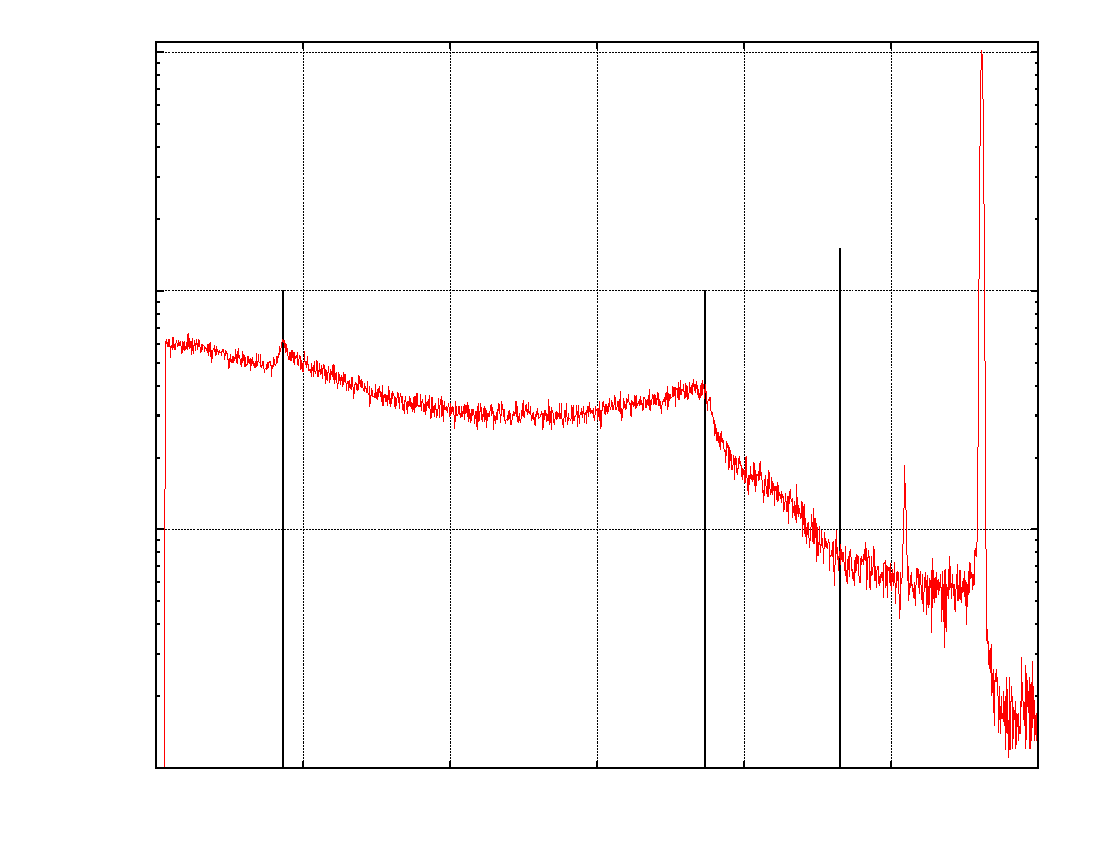
\includegraphics{cs_sp}}%
    \gplfronttext
  \end{picture}%
\endgroup

\caption{Aparaturní spektrum \pr{137}{Cs}}
\label{g:cs_sp}
\end{graph}

\subsection*{\pr{24}{Na}+\pr{36}{Cl}}
Energie FEP1 byla \peak{1368.62}{0.02}{0.10} \fw{2.27}. 

Energie FEP2 byla \peak{2754.15}{0.03}{0.10} \fw{2.80}. 

Energie SEP2 \peak{2243.10}{0.05}{0.10} \fw{2.96}. 

Energie DEP2 \peak{1732.01}{0.04}{0.10} \fw{2.72}.

Pro FEP1 byla comptonova hrana byla na \rozmezi{1129}{1160} a druhá na \rozmezi{1244}{1290}.

Pro FEP2 byla comptonova hrana byla na \rozmezi{2500}{2530} a druhá na \rozmezi{2625}{2670}.

Anihilační pík měl energii \peak{510.50}{0.07}{0.10} \fw{3.13}.

Hranu zpětného rozptylu se nám nepodařilo najít. V grafu \ref{g:nacl_sp} je jako "zpětný rozptyl" vyznačena hodnota změřená u \pr{137}{Cs}, protože by se od ní neměla přiliš lišit \cite{skripta}. Pík označený jako "přirozené pozadí" je stejný pík na cca \kev{610} jako v grafu \ref{g:cs_sp}.

\begin{graph}[htbp] 
\centering
% GNUPLOT: LaTeX picture with Postscript
\begingroup
  \makeatletter
  \providecommand\color[2][]{%
    \GenericError{(gnuplot) \space\space\space\@spaces}{%
      Package color not loaded in conjunction with
      terminal option `colourtext'%
    }{See the gnuplot documentation for explanation.%
    }{Either use 'blacktext' in gnuplot or load the package
      color.sty in LaTeX.}%
    \renewcommand\color[2][]{}%
  }%
  \providecommand\includegraphics[2][]{%
    \GenericError{(gnuplot) \space\space\space\@spaces}{%
      Package graphicx or graphics not loaded%
    }{See the gnuplot documentation for explanation.%
    }{The gnuplot epslatex terminal needs graphicx.sty or graphics.sty.}%
    \renewcommand\includegraphics[2][]{}%
  }%
  \providecommand\rotatebox[2]{#2}%
  \@ifundefined{ifGPcolor}{%
    \newif\ifGPcolor
    \GPcolortrue
  }{}%
  \@ifundefined{ifGPblacktext}{%
    \newif\ifGPblacktext
    \GPblacktextfalse
  }{}%
  % define a \g@addto@macro without @ in the name:
  \let\gplgaddtomacro\g@addto@macro
  % define empty templates for all commands taking text:
  \gdef\gplbacktext{}%
  \gdef\gplfronttext{}%
  \makeatother
  \ifGPblacktext
    % no textcolor at all
    \def\colorrgb#1{}%
    \def\colorgray#1{}%
  \else
    % gray or color?
    \ifGPcolor
      \def\colorrgb#1{\color[rgb]{#1}}%
      \def\colorgray#1{\color[gray]{#1}}%
      \expandafter\def\csname LTw\endcsname{\color{white}}%
      \expandafter\def\csname LTb\endcsname{\color{black}}%
      \expandafter\def\csname LTa\endcsname{\color{black}}%
      \expandafter\def\csname LT0\endcsname{\color[rgb]{1,0,0}}%
      \expandafter\def\csname LT1\endcsname{\color[rgb]{0,1,0}}%
      \expandafter\def\csname LT2\endcsname{\color[rgb]{0,0,1}}%
      \expandafter\def\csname LT3\endcsname{\color[rgb]{1,0,1}}%
      \expandafter\def\csname LT4\endcsname{\color[rgb]{0,1,1}}%
      \expandafter\def\csname LT5\endcsname{\color[rgb]{1,1,0}}%
      \expandafter\def\csname LT6\endcsname{\color[rgb]{0,0,0}}%
      \expandafter\def\csname LT7\endcsname{\color[rgb]{1,0.3,0}}%
      \expandafter\def\csname LT8\endcsname{\color[rgb]{0.5,0.5,0.5}}%
    \else
      % gray
      \def\colorrgb#1{\color{black}}%
      \def\colorgray#1{\color[gray]{#1}}%
      \expandafter\def\csname LTw\endcsname{\color{white}}%
      \expandafter\def\csname LTb\endcsname{\color{black}}%
      \expandafter\def\csname LTa\endcsname{\color{black}}%
      \expandafter\def\csname LT0\endcsname{\color{black}}%
      \expandafter\def\csname LT1\endcsname{\color{black}}%
      \expandafter\def\csname LT2\endcsname{\color{black}}%
      \expandafter\def\csname LT3\endcsname{\color{black}}%
      \expandafter\def\csname LT4\endcsname{\color{black}}%
      \expandafter\def\csname LT5\endcsname{\color{black}}%
      \expandafter\def\csname LT6\endcsname{\color{black}}%
      \expandafter\def\csname LT7\endcsname{\color{black}}%
      \expandafter\def\csname LT8\endcsname{\color{black}}%
    \fi
  \fi
  \setlength{\unitlength}{0.0500bp}%
  \begin{picture}(10204.00,7936.00)%
    \gplgaddtomacro\gplbacktext{%
      \csname LTb\endcsname%
      \put(946,704){\makebox(0,0)[r]{\strut{} 0}}%
      \csname LTb\endcsname%
      \put(946,2097){\makebox(0,0)[r]{\strut{} 100}}%
      \csname LTb\endcsname%
      \put(946,3491){\makebox(0,0)[r]{\strut{} 200}}%
      \csname LTb\endcsname%
      \put(946,4884){\makebox(0,0)[r]{\strut{} 300}}%
      \csname LTb\endcsname%
      \put(946,6278){\makebox(0,0)[r]{\strut{} 400}}%
      \csname LTb\endcsname%
      \put(946,7671){\makebox(0,0)[r]{\strut{} 500}}%
      \csname LTb\endcsname%
      \put(2329,484){\makebox(0,0){\strut{} 500}}%
      \csname LTb\endcsname%
      \put(3894,484){\makebox(0,0){\strut{} 1000}}%
      \csname LTb\endcsname%
      \put(5458,484){\makebox(0,0){\strut{} 1500}}%
      \csname LTb\endcsname%
      \put(7022,484){\makebox(0,0){\strut{} 2000}}%
      \csname LTb\endcsname%
      \put(8587,484){\makebox(0,0){\strut{} 2500}}%
      \put(176,4187){\rotatebox{-270}{\makebox(0,0){\strut{}výtěžek}}}%
      \put(5442,154){\makebox(0,0){\strut{}$E$ (\si{\keV})}}%
      \put(5020,6556){\makebox(0,0)[r]{\strut{}FEP1}}%
      \put(6184,3351){\makebox(0,0){\strut{}DEP2}}%
      \put(7783,1958){\makebox(0,0){\strut{}SEP2}}%
      \put(9382,5163){\makebox(0,0){\strut{}FEP2}}%
      \put(2362,2794){\makebox(0,0){\strut{}anih.}}%
      \put(2670,4188){\makebox(0,0){\strut{}\shortstack{přirozené\\prostředí}}}%
      \put(1422,6417){\makebox(0,0)[l]{\strut{}zpětný rozptyl}}%
      \put(4832,3769){\makebox(0,0)[r]{\strut{}\shortstack{comptonovy\\hrany (FEP1)}}}%
      \put(9119,3769){\makebox(0,0)[r]{\strut{}\shortstack{comptonovy\\hrany (FEP2)}}}%
    }%
    \gplgaddtomacro\gplfronttext{%
    }%
    \gplbacktext
    \put(0,0){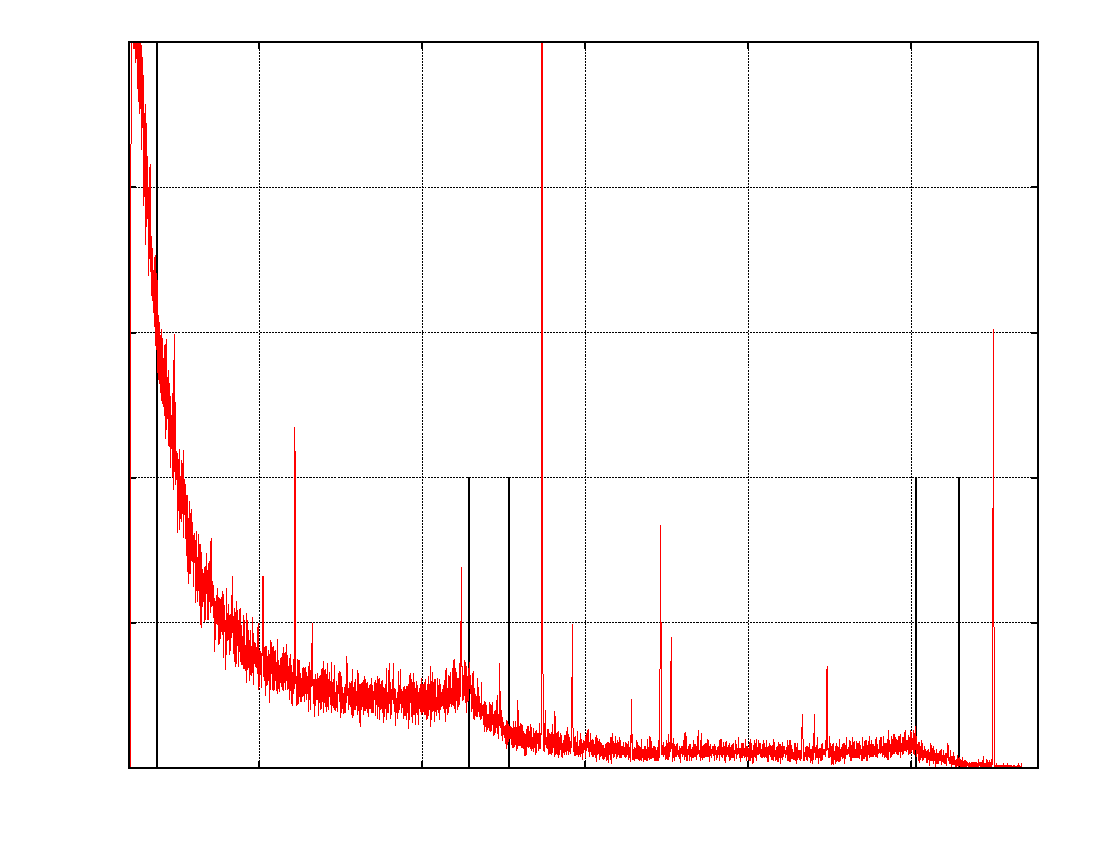
\includegraphics{nacl_sp}}%
    \gplfronttext
  \end{picture}%
\endgroup

\caption{Aparaturní spektrum \pr{24}{Na}+\pr{36}{Cl}}
\label{g:nacl_sp}
\end{graph}